\chapter{Estimating How Well a Design Will Scale}
%\chapter{The Maximum Room For Improvement Metric}
%\chapter{Assessing Scalability}
\label{chapter:estimating-scalability}

It would be nice to be able to predict how well a data model design and
implementation will scale up, as you increase the complexity or number of
entities. The bloat factor of a data structure tells you, for a given size, what
fraction of its size is overhead versus actual data. To judge whether it will
scale requires extrapolating these costs out. This chapter introduces a metric,
and some facilitating techniques, that enable you to more quickly make these
predictions. The metric is called the Maximum Room for Improvement\index{Maximum
Room for Improvement}, which is the highest factor of improvement in scalability
you can expect to wring out of a given design, after all possibly amortizable
costs have been amortized away.

\section{The Asymptotic Nature of Bloat}
Up till now, bloat factor has been treated as a scalar quantity: e.g., 95\% of
space is devoted to implementation overhead rather than actual data. More
accurately, the bloat factor of a data structure is a function of its size. The
bloat factor of a collection of objects decreases until it reaches an
\emph{asymptote}, the lowest bloat factor a data structure car achieve, no
matter how big it grows.

%%%%%%%%%%%%%%%%%%%%%%%%%%%%%%%%%%%%%%%
%%%% ASYMPTOTIC BLOAT FACTOR CALLOUT
%%%%
\callout{asymptoticbloatfactor}{Data Structure Scaling: Asymptotic Bloat
Factor}{A data structure scales well, or not, depending upon how its bloat
factor changes as it grows. It starts by decreasing, as the collection's fixed
costs are amortized over a larger amount of actual data, and soon levels off.
This \emph{asymptotic bloat factor} is governed by the collection's
variable cost and the bloat factor and \emph{unit cost} of the contents.}
%%%%
%%%% ASYMPTOTIC BLOAT FACTOR CALLOUT
%%%%%%%%%%%%%%%%%%%%%%%%%%%%%%%%%%%%%%%

\autoref{fig:asymptotic-bloat-factor} illustrates an example of the asymptotic
behavior of bloat factor for two collection types. With a small number of
elements, the fixed costs dominate. For this example, for a \class{HashMap},
with more than about 10 elements, fixed costs are pretty much fully amortized;
the fixed cost of a \class{ConcurrentHashMap} requires more elements to amortize
away. In either case, at this point, the bloat factor of the elements being
stored in the collection, along with the collection's variable costs, become the
dominant factors. In this example, the total cost per element is 128 bytes, 64
bytes of which is overhead. Ultimately, it is that ratio of 64/128, or 0.5,
which governs the asymptotic bloat factor of this structure.


\begin{figure}
\centering
% source is in bytesPerEntity.numbers
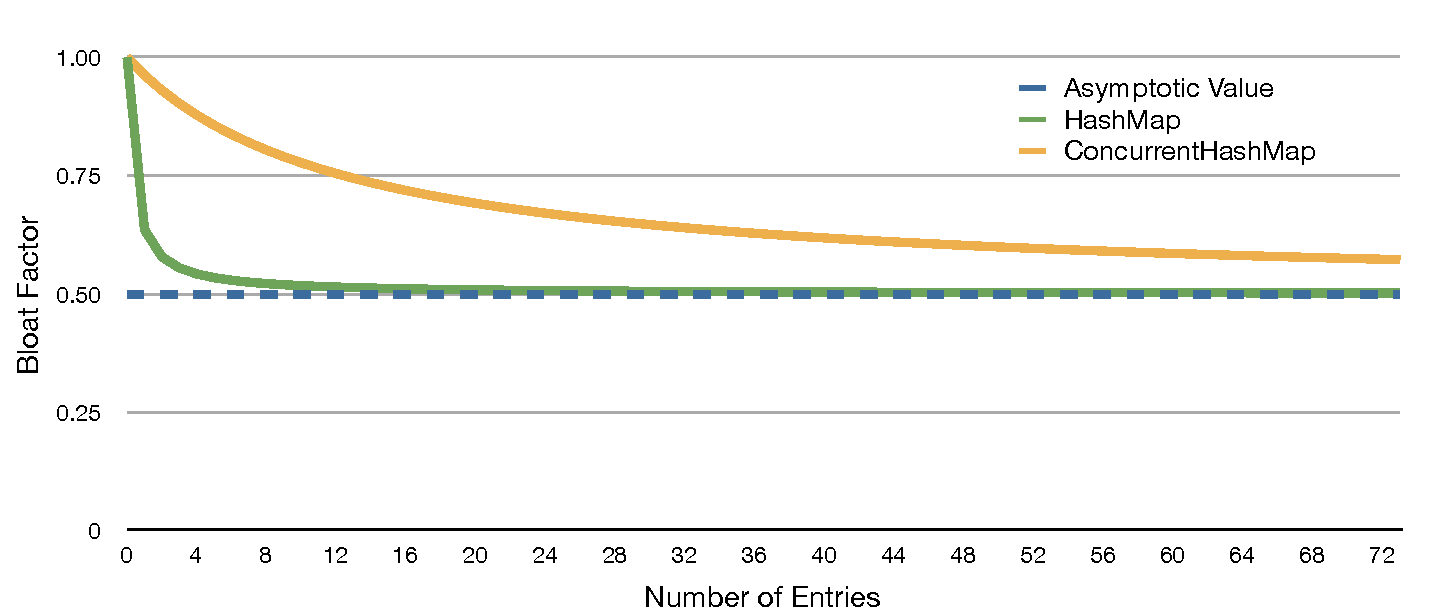
\includegraphics[width=0.8\textwidth]{part3/Figures/assessing/asymptote}
\caption{An example of the asymptotic behavior of bloat factor.}
\label{fig:asymptotic-bloat-factor}
\end{figure}

\paragraph{Amortizing Fixed Costs}
Data structures that can change in size, as opposed to having a fixed size,  do
so because they make use of collection. As you learned in \autoref{part:1},
collections of objects have a \emph{fixed cost} that is independent of the
number of entries in contains. For a simple array, this is the \jre object
header. For more complex collections of objects, such as
\class{java.util.HashSet}, the fixed cost includes a extra wrapper cost. This
fixed cost is quickly amortized, usually once the data structure grows to have
more than a dozen or two elements.

The number of elements that it takes to amortize a collections fixed cost
depends on that cost in comparison to the memory cost of storing elements. If
the collection's fixed cost is 48 bytes, and it costs 128 bytes per stored
element, then the collection must have at least 6 elements before the fixed
overhead contributes less than 5\% to the overall size of the collection:

$$\frac{\textrm{collection fixed cost}}{\textrm{collection total cost}} =
\frac{48}{48 + 128 N} \le 0.05 \Longrightarrow N \ge 5.45$$

Once fixed costs have largely amortized, the asymptotic bloat factor is reached.
For this reason, at least for collections that you expect to be at least
moderately sized, it is the asymptotic bloat factor that should be your primary
concern.

\paragraph{Unit Costs}
However, the fixed costs of collections still play an important role in the
ultimate scalability of most data structure. When one collection is nested
inside of another, the fixed cost of nested collection contributes to the
\emph{unit cost} of storing things in the outer collection.

%%%%%%%%%%%%%%%%%%%%%%%%%%%%%
%%%% UNIT COST CALLOUT
%%%%
\callout{unitcost}{The Unit Cost of Storing Data in Collections}{
\begin{wrapfigure}{r}{0.3\textwidth}

%% this is necessary to get the figure to appear within the callout
\vspace{-17pt}

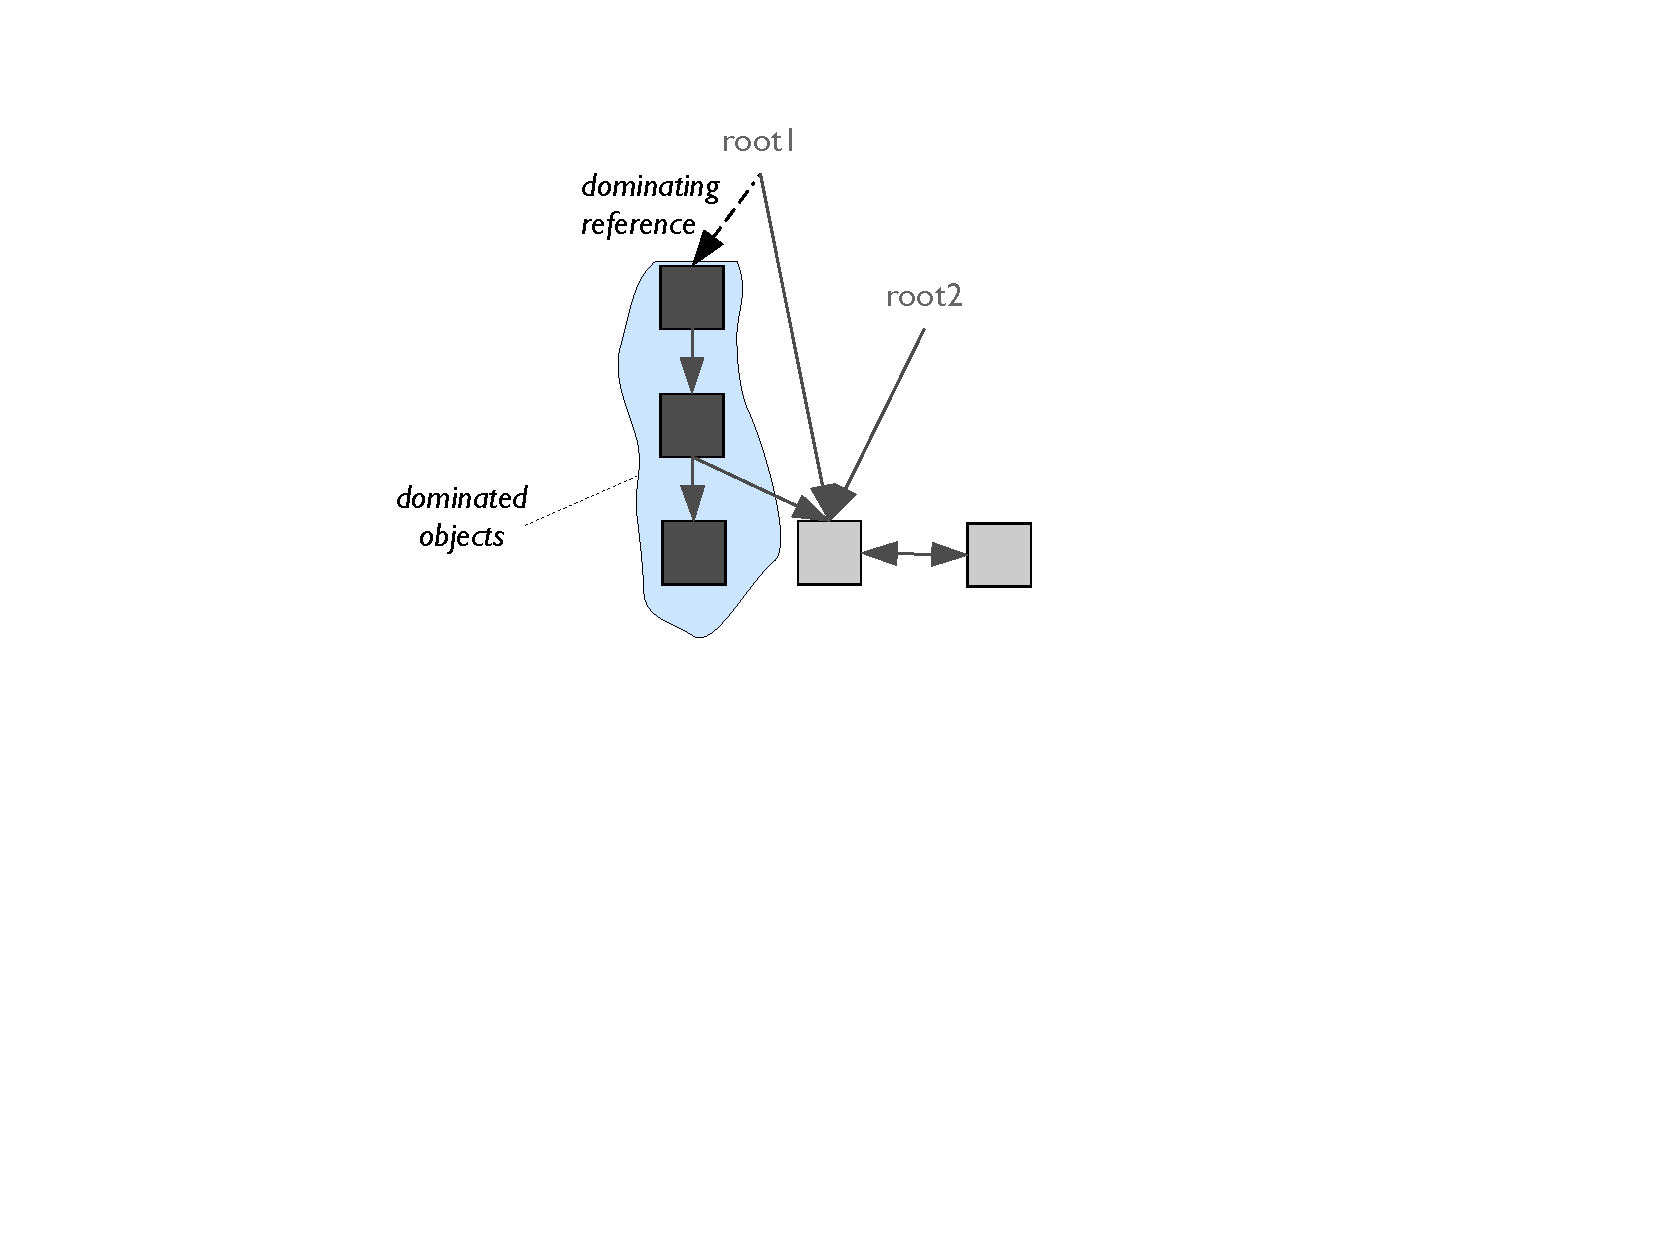
\includegraphics[width=0.3\textwidth]{part2/Figures/lifetime/reachability2}
\end{wrapfigure}
The \emph{unit cost} of storing elements in a collection is the average size of
each contained element. This cost includes everything uniquely owned by the
elements. See \autoref{sec:dominance} for more discussion of \emph{dominance},
which is a property of a graph of objects as illustrated on the right. }
%%%%
%%%% UNIT COST CALLOUT
%%%%%%%%%%%%%%%%%%%%%%%%%%%%%

Every class has a \emph{unit cost}, the cost for every additional instance. You
can determine the unit cost of a class by counting up the size of its fields,
taking into account \jre-imposed costs. Similarly, every interconnected group of
instances has a unit cost, the sum of the sizes of the classes involved in that
group. \autoref{sec:CostOfObjects} introduced this style of accounting.
\autoref{fig:ec-scalability-example} gives an example EC diagram of a HashMap
that contains an interconnected group of four objects. The unit cost of each
entry in this structure is given by the sum of the sizes of those classes: 88
bytes, in this case.
\begin{wrapfigure}{l}{0.45\textwidth}
\centering
% source is in heaps_and_stacks.odg
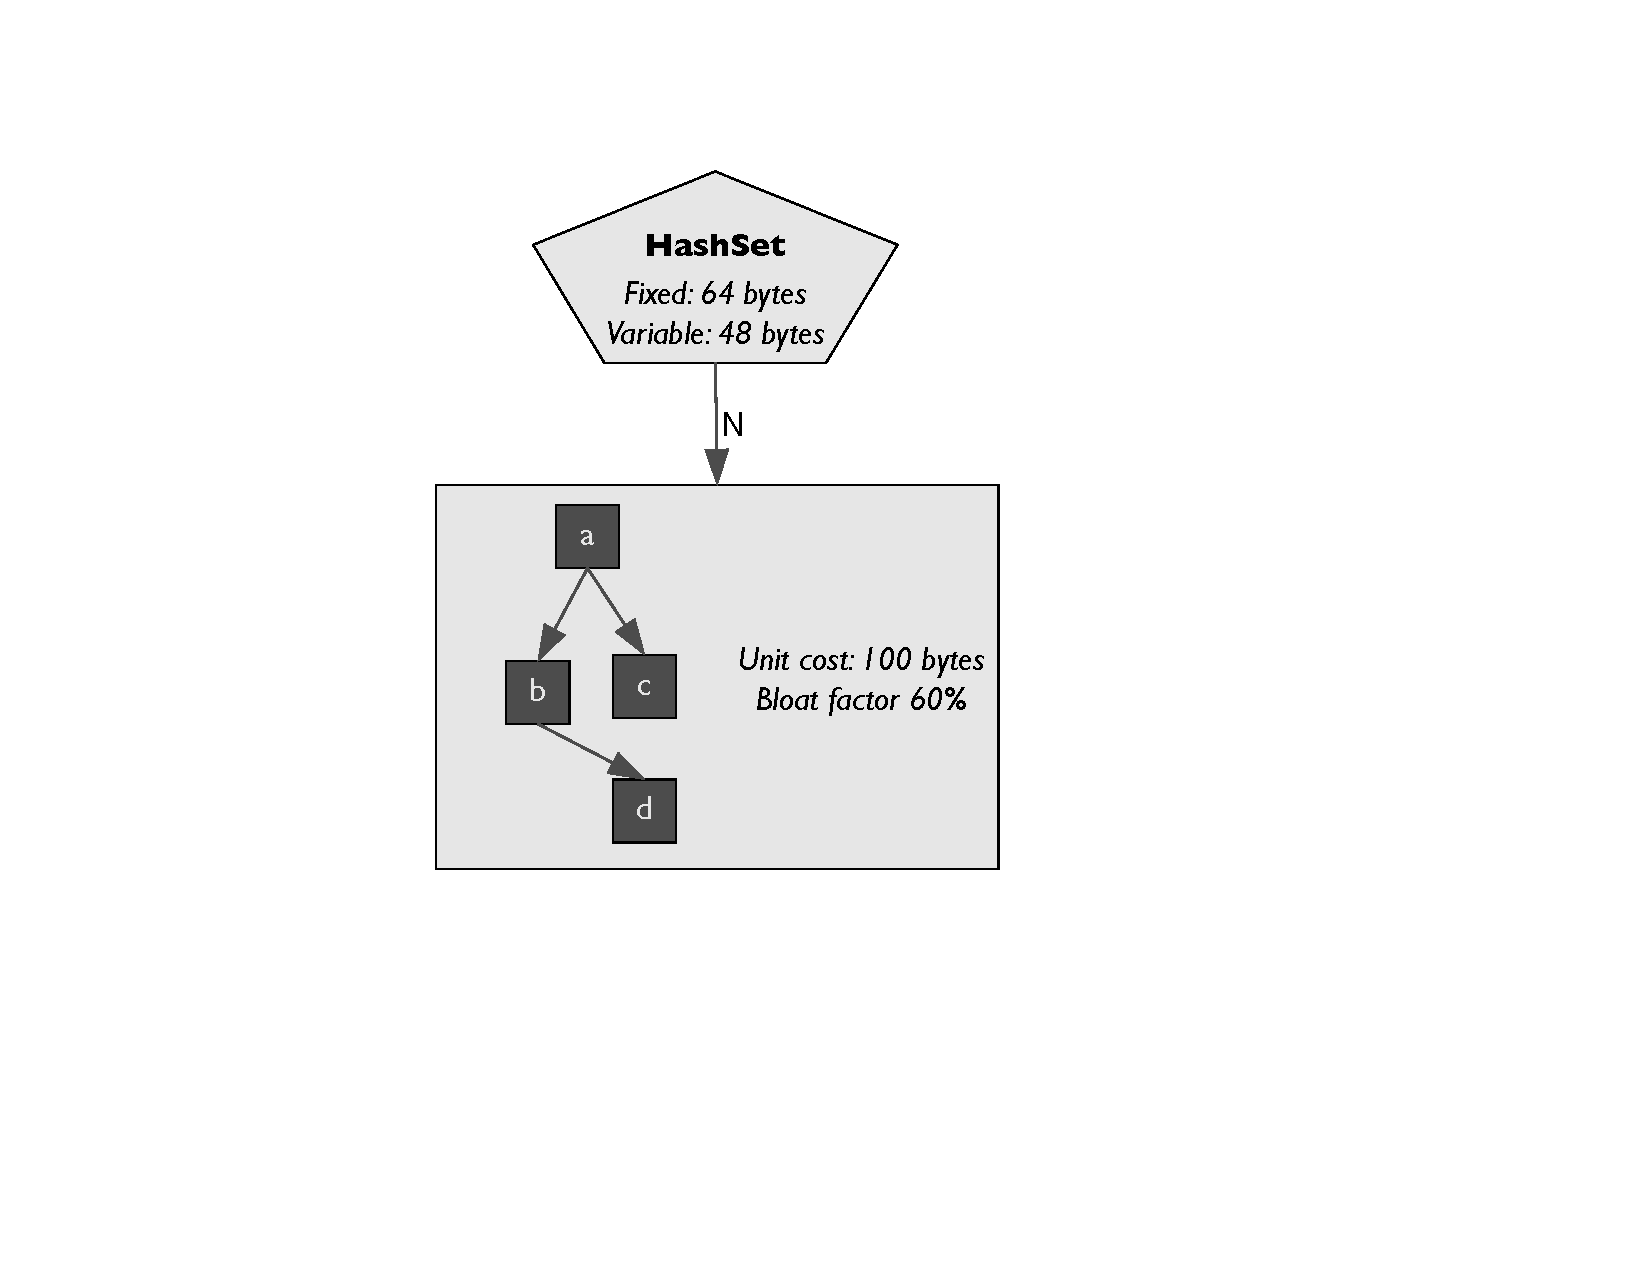
\includegraphics[width=0.45\textwidth]{part3/Figures/assessing/EC-example}
\caption{EC diagram for a \class{HashSet} that contains data structures, each
composed of four interconnected objects.}
\label{fig:ec-scalability-example}
\end{wrapfigure}

Quite often, the elements you are adding themselves consist of nested
collections. If you don't expect those nested collections to grow, then they
contribute to the unit cost of additional elements in the structure that
\emph{is} growing. A fixed-size collection has a unit cost which is that
collection's fixed cost, plus the total size of all of the variable costs and
unit costs, counted once for each entry. So, if you have a fixed-size collection
with four entries, then the total cost is the fixed cost plus four times the sum
of the variable costs of the collection plus the unit cost of what's inside.


\paragraph{Determining the Maximum Room For Improvement}
\autoref{fig:ec-scalability-example} is annotated with the four numbers that
govern the scalability of this structure: the fixed and variable costs of the
collection you use, and the unit cost and bloat factor of the data you're
storing inside of it. The maximum room for improvement of a
collection of data structures is given by:
\begin{align*}
V &= \textrm{collection variable cost} \\
U &= \textrm{unit cost of actual data} \\
B &= \textrm{bloat factor of contained structures} \\
\textbf{\textrm{maximum room for improvement}} &= \frac{V}{U} + \frac{1}{1-B}
\end{align*}

For example, the variable cost of a \class{HashMap} is 48 bytes. If you're
storing structures with a unit cost of 40 bytes each with a bloat factor of
50\%, then the maximum room for improvement is $\frac{48}{40} + \frac{1}{1-0.5}$
or 3.2x. This means that there is a fairly good scalability benefit you'll see from
tuning.

%A similar accounting is possible to help you estimate how a collection of
%objects will grow in size as elements are added. Every additional element added
%to a collection costs the collection's variable cost plus the unit cost of the
%added element. 

\paragraph{Will It Fit? Should I Tune?}

From unit costs and the maximum room for improvement, you can estimate answers
to the these two important scalability questions. If you have a fixed amount of heap
size that each process has access to, then your data model designs will fit if
memory capacity divided by unit cost, which is the number of elements you can
afford, is at least as large as you need. For example, if you have one gigabyte
of memory available, and each user comes with a unit cost of one megabyte, then
you can support at most 1000 simultaneous users. Is this enough? 

If not, then you have two options: buy more hardware, or tune. If possible, you
could buy more memory, or more machines if your current machines cannot accept
any more physical memory. You must also pay attention to address space limits,
as discussed in \autoref{sec:address-space}: if your 32-bit processes cannot fit
anything more into the constrained address space, then the answer to ``Will It
Fit?'' is no! In this case, buying more physical memory won't help, and your only
option is to tune your data models.

\begin{figure}
\callout{when-to-tune}{Rule of Thumb: When Should I Bother Tuning?}{
A good rule of thumb to following, when deciding whether to tune or to buy more
hardware in order to increase scalability, is to look at the asymptotic bloat
factor of your dominant structures. For each data structure that are expected
to grow the largest, tune it only when its asymptotic bloat factor is above
50\%. You can estimate which structures are the dominant ones by looking at
the unit cost of each, and multiplying these figures out by how many elements
you'd like to have in each.}
\end{figure}

The maximum room for improvement of your dominant data structures can help you
to understand whether you should bother tuning. If a data structure has a low bloat
factor, then there isn't much bloat to optimize away. For example, in a web
application server, session state will scale up roughly depending on the number
of concurrent users. If the unit cost per user is one megabyte, and you'd like
to support 1000 concurrent users, then this is clearly a dominant structure. If
you can't afford one gigabyte for session state, then and if the bloat factor of
your session state data models is greater than 50\%, then you should consider
tuning these models.

\section{Quickly Estimating the Scalability of an Application}

It can be tedious to construct formulas in order to estimate the scalability of
your data models. Estimating scalability can require navigating a space with
many dimensions of freedom. Sometimes, you have a fixed amount of memory, and a
fixed amount of actual data to store, and want to know how much you need to
tune, in order to make it fit. Sometimes, you have some flexibility in how much
data you're keeping around. Luckily, there are some simplyfing studies that you
can do, where you fix certain parameers, and let others vary.
\autoref{fig:maxActualData} and \autoref{fig:maxBloatFactor} show two of these.
In both cases, the amount of memory available is fixed at one gigabyte. The
first chart plots how much actual data you can afford to keep around, for
various degrees of bloat (the four level curves). The second chart plots how
high an asymptotic bloat factor you can afford, for various amounts of actual
data (the four level curves). For many cases, you can simply consult these
charts. However, it isn't difficult to construct your own, as described in
\autoref{fig:deriving-scalability-formulas}.


\begin{figure}
\centering
    \subfigure[The amount of actual data you can store in your entities depends on
	the degree of delegation in your entities, and the per-entry overhead of the collection in which these entities
	reside.]{
       \label{fig:maxActualData}
	   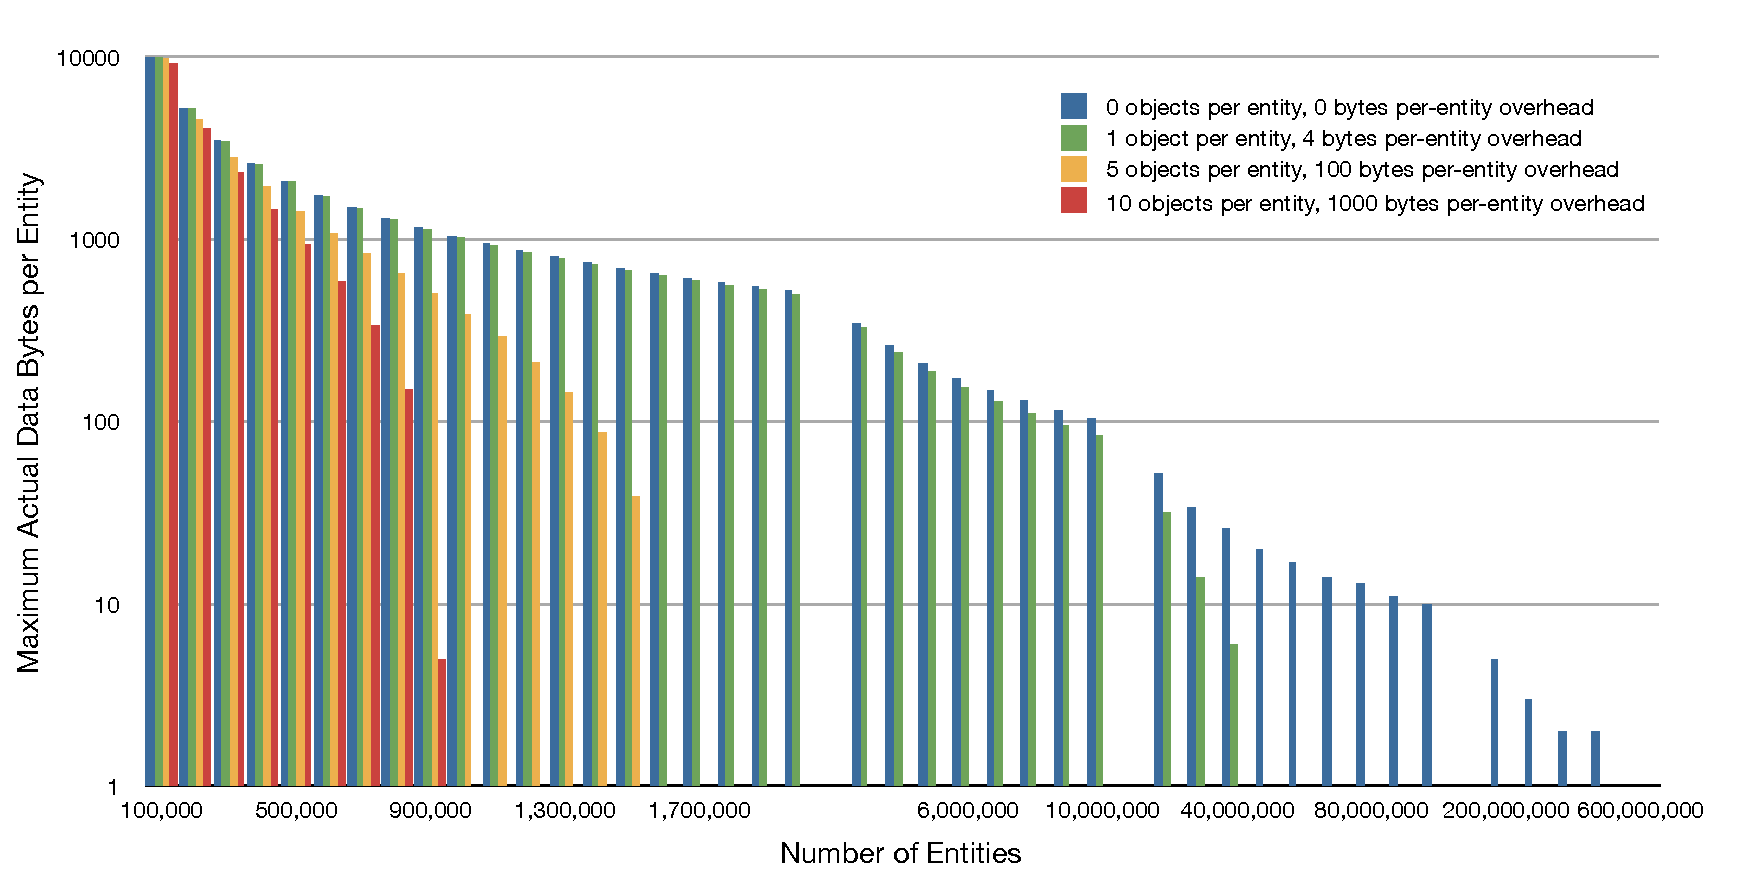
\includegraphics[width=\textwidth]{part3/Figures/assessing/maxActualData}
	}

% C is megabytes of memory available A is number of entitles D is unit cost of
% actual data x is the unknown bloat factor C*1024*1024/A / (1/(1-x) * D)) >= 1
% x <= 1-A*D/(C*1024*1024)
    \subfigure[The area under each curve shows the bloat factor you can afford,
    for various amounts of actual data that you need to store.]{
	   \label{fig:maxBloatFactor}
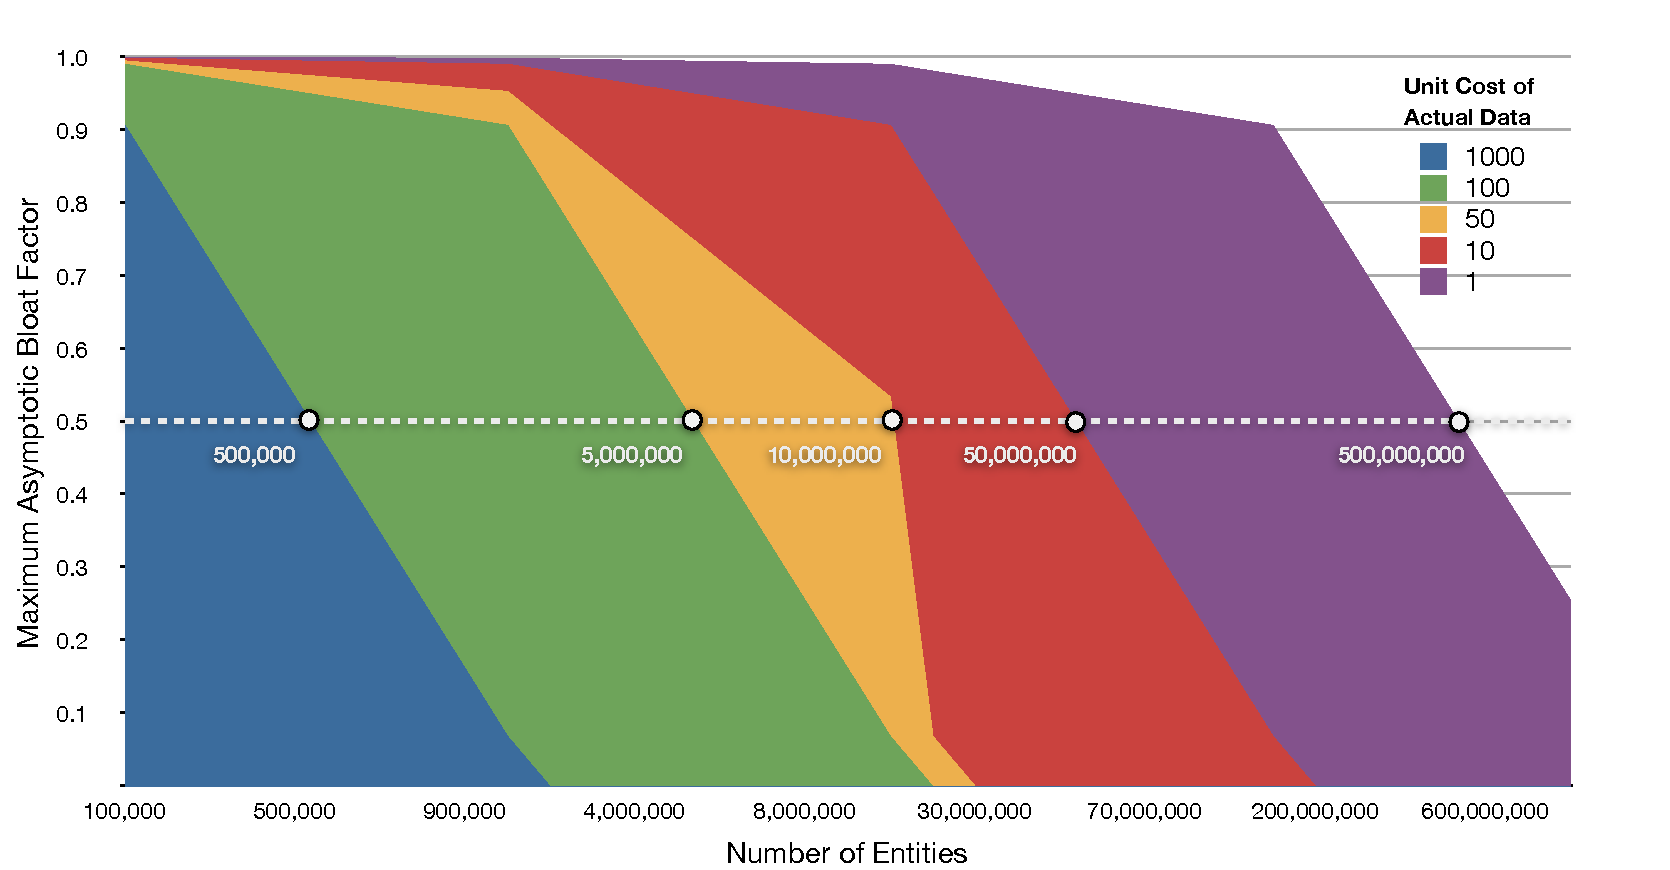
\includegraphics[width=\textwidth]{part3/Figures/assessing/maxBloatFactor} }
   \caption{You can consult these charts to get a quick sense of where your
   design fits in the space of scalability. These charts are based upon having 1
   gigabyte of Java heap. Note the logarithmic scale of the horizontal axis.}
\end{figure}


\begin{figure}
\callout{ezscalability}{Deriving Scalability Formulas \hfill [For Experts]}{
It isn't hard to make your own scalability charts, with some simple algebra
and your favorite spreadsheet software. Before you can plot anything, you
will need to construct a formula that governs how things scale. Consider the chart in
\autoref{fig:maxBloatFactor},
which 
plots the bloat factor that will let you fit \emph{at
least} one element of data in memory.
The formula behind this chart depends upon these quantities: let $M$ be the
bytes of memory available, $N$ be the number of entities, and $D$ be the unit cost of your actual data, and
$x$ be the unknown maximum room for improvement that you need to solve for.

The \emph{maximum} number of bytes per entity you can afford is the ratio of
memory capacity to the number of entities: $M/N$. The exact cost per entity,
including overhead is $\frac{1}{1-x} D$; e.g. 20 bytes of actual data with a
bloat factor of 60\% means the total size per entity is 50 bytes. 
%(because $50 - 50 * 0.6 = 20$).
% \begin{align*}
$$\frac{M}{N} \ge \frac{1}{1-x} D
 %\\
% \frac{M (1-x)}{N D}  &\ge 1
% \\
% 1-x  &\ge \frac{N D}{M}
% \\
~~~~\Longrightarrow~~~~ x  \le 1-\frac{N D}{M} $$
% \end{align*}
}
\label{fig:deriving-scalability-formulas}
\end{figure}

\section{Example: Designing a Graph Model for Scalability}

Let's step through an example of getting a data model to scale. This extended
example focuses on modeling relationships between entities, like the employees
within a department, or the books on a certain topic. This is a modeling task
you face whenever bringing in data from some relational data store, loading in
trace or log data, or modeling XML information. There are many examples that
fall into this general space.

This is a task you'll often face, but getting a relational data model design to
scale is hard. Database developers from Oracle, IBM, and others, have worked for
decades to tune the way their databases store this kind of information. When
this data is loaded into Java, we all pay much less attention to the way that
same data is laid out in the Java heap. A general-purpose storage strategy,
using Java objects in the natural way, is very likely not to scale well.
% To achieve good scalability usually requires optimizing for the ways in which
% the data will be used by other parts of your application.
Something you should keep in mind is that, at each step along the way, as you
tune your data model for certain use cases, is to keep a focus on the two
important aspects of scalability: unit costs and asymptotic bloat factor. These
factors will determine the scalability success of your design.

\paragraph{Modeling Relationships Means Modeling Graphs}
Representing relationships between entities is no different than representing a
graph of nodes and edges: entities are nodes, and relationships are edges. A
small graph is illustrated in \autoref{fig:example-storing-relations-graph}.
When caching data from a relational database in the Java heap, each
database row is an entity. Columns containing numbers, dates, string, and binary
large objects (BLOBs) data are all attributes of these entities. So far, the way
you'd store this entity information in Java is somewhat similar to the way you'd
store things in a relational database.


\begin{wrapfigure}{r}{0.34\textwidth}
    %\vspace{-5mm}
    \centering
	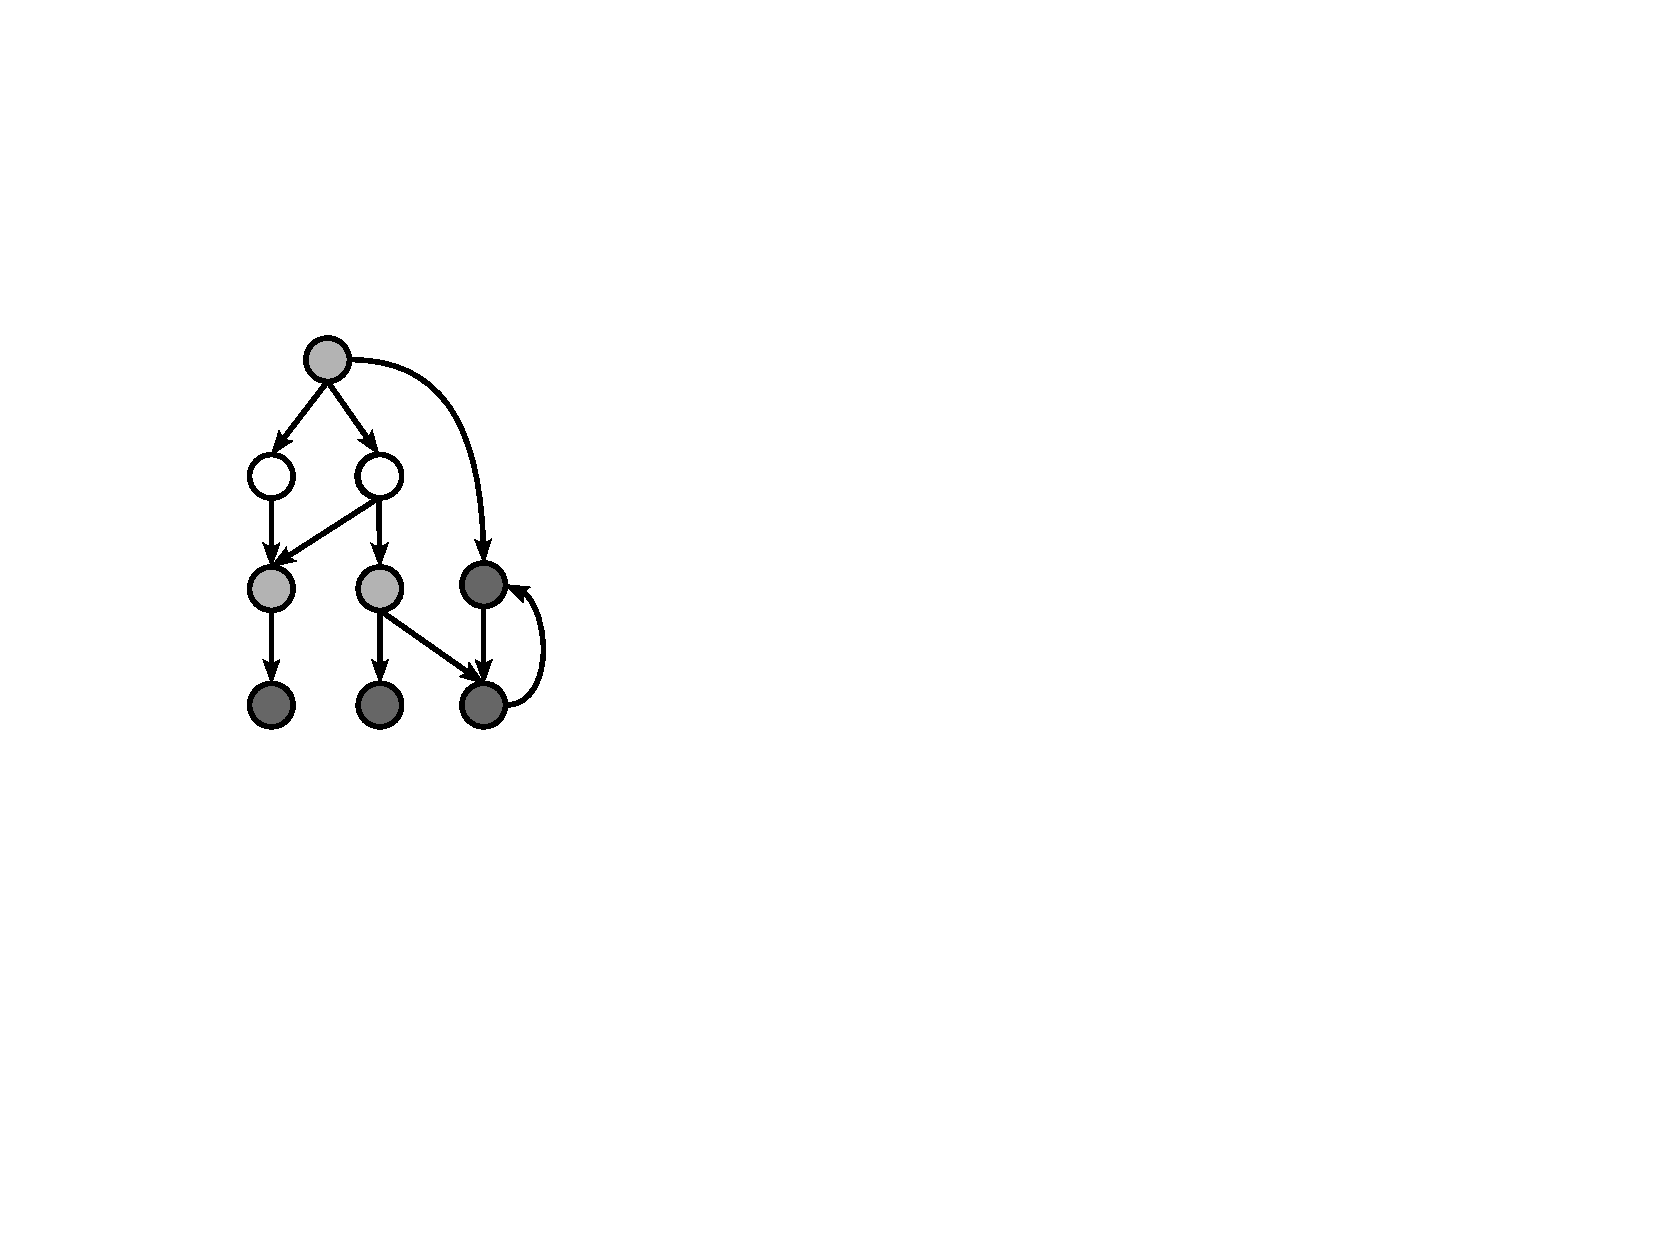
\includegraphics[width=0.3\textwidth]{part3/Figures/assessing/exampleGraph}
	\caption{Example graph.}
    \label{fig:example-storing-relations-graph}
\end{wrapfigure}

Storing relationships is where things start to diverge. In Java, it is natural
to store the relationship information, such as the employees under a manager, as
references to collections of other entities: a manager object points to a set of
employee objects. In a database, this information is usually stored in a
separate table; e.g. a table that maps managers to the employees they supervise.
In Java, this isn't a very natural way to model things.
% The Java heap itself is a graph of objects, and so storing a graph of entities
% and relations as a graph of objects is a natural, though possibly inefficient,
% mapping of relational data into Java classes and fields. If a graph has a
% great many nodes and edges, you must design its storage carefully. 

The implementation strategy you choose depends heavily upon the use cases that
you need to handle. Do your edges have properties, such as an edge weight? Do
you need random access to the edges? Do you need edges at all, or only nodes
along with edge fanouts? How will you be traversing the edges? The Java
interfaces help to shape your implementation to these use cases.

Every interface fixes some things, while sitll allowing some degree of freedom
in the implementation. \autoref{fig:graph-interfaces} shows two interfaces that
this example will work through. In one case, there are no edge properties, and
in the second case, each edge as an associated weight. If your edges don't have
any properties associated with them, then there is no need for an \class{IEdge}
interface. 

\begin{figure}
\centering
\begin{subfloat}
\label{fig:graph-interfaces}
\begin{minipage}[b]{0.45\textwidth}
%interface IGraph {
	%Set<Node> getNodes();
%}
\begin{framedlisting}
interface INode {
  Color color();
  Collection<INode> children();
  Collection<INode> parents();
}
enum Color {
  White, LightGray, DarkGray
}
\end{framedlisting}
\end{minipage}
\caption{If you don't need edge properties.}
\end{subfloat}
%\qquad
\begin{subfloat}
\label{fig:graph-interfaces}
\begin{minipage}[b]{0.45\textwidth}
%interface IGraph {
   %Set<Node> getNodes();
   %Set<Edge> getEdges();
%}
\begin{framedlisting}
interface INode {
  Color color();
  Collection<IEdge> children();
  Collection<IEdge> parents();
}
interface IEdge<Property> {
   Property property();
   INode from();
   INode to();
}
\end{framedlisting}
\end{minipage}
\caption{If you do!}
\end{subfloat}
\caption{Java interfaces that define the abstract data types for nodes and
edges.}
\label{fig:graph-interfaces}
\end{figure}

%There are several ways to implement the abstract data types, of nodes and
%edges. Each strategy has its positives and negatives, depending on which of
%ease of maintenance or memory consumption is of primary importance.

\subsection{The Straightforward Implementation, and Some Tweaks}
\label{sec:graph-straightforward}
A reasonable place to start is with a straightforward mapping of interfaces to
concrete classes.
\autoref{fig:node-obvious-impl} shows such an implementation for the
\class{Node} data type.
Following this strategy, the \class{Node} class has three fields, one to store
its \class{Color}, and two for the relations to children and parents. These two
relations are implemented with a standard \class{HashSet} collection. In the
case where the design requires edge properties, there is an \class{Edge} class
with one field that stores the edge property, and two reference fields that
store the source and target nodes.

This is a pretty natural expression of a graph in Java, and it's easy to
implement and maintain. There are no corner cases to handle, in terms of adding
or removing nodes or edges. It's easy for new project members to map between
interface and implementation, because the two are parallel versions of each
other. The nodes and edges, and relations between them, are objects that can be
manipulated using normal object oriented practices; e.g. you can write
\texttt{node.children().get(5).getTo()\-.color()} and, later, quickly
understand what is going on. Contrast this with interacting with a
non-object-oriented data storage, such as
memcached\index{memcached}\cite{memcached} or a relational database. To access
an attribute in this non-OO data would be more work, and would not read as
cleanly.\footnote{There are frameworks that hide the details of accessing this
information, such as Hibernate\cite{hibernate}. Under the covers, though, the
same mismatch exists, and now you are faced with the added complexities of
interacting with these APIs.}

\begin{figure}
\centering
\begin{subfloat}
\begin{minipage}[b]{0.59\textwidth}
\begin{framedlisting}
class Node<E> {
   Color color;
   Set<E> parent = new HashSet<E>();
   Set<E> children = new HashSet<E>();
}
\end{framedlisting}
\end{minipage}
\caption{Node implementation.}
\end{subfloat}
%\quad
\begin{subfloat}
\begin{minipage}[b]{0.33\textwidth}
\begin{framedlisting}
class Edge<Property> {
   Property property;
   Node<Edge> from, to;
}
\end{framedlisting}
\end{minipage}
\caption{Edge implementation, if you have edge properties.}
\end{subfloat}
\caption{A straightforward implementation of the \class{INode} interface,
one that is parameterized the type used for parents and
children; e.g. a node without edge properties would be a subclass of
\class{Node<Node>}, because the parents and children point directly to other
nodes.}
\label{fig:node-obvious-impl}
\end{figure}

In this implementation, the unit cost per node is three pointers plus two
collections of default size. If a typical node has one parent and two children,
then the unit cost of a node will be $404$ bytes: one object header, plus three
pointer fields, plus two 136-byte collection fixed costs, plus three 28-byte
collection variable costs (\autoref{tab:collection-costs} shows the fixed and
variable costs of standard collections). At this unit cost, you can fit at most
2.6 million nodes into one gigabyte of Java heap. Is it worth tuning? That
depends on the maximum room For improvement of this design, as things scale up.

Every node stores 16
bytes of actual data (its color, parent, and two children), compared to its 380
byte total unit cost. Let's assume that the nodes are stored in a simple array.
From these values, we can compute the maximum room for improvement:
\begin{align*}
V &= 4 ~~~~~~~~~~~~~~~~~\textrm{(variable cost of node array)}\\
U &= 16 ~~~~~~~~~~~~~~~\textrm{(actual data per node)}\\
B &= 1-16/380 ~~~~\textrm{(bloat factor of node)}\\
\textbf{\textrm{maximum room for improvement}} &= \frac{V}{U} + \frac{1}{1-B} =
24x
\end{align*}
The maximum room for improvement is a factor of 24x, which is very high.
\autoref{tab:graph-mri} tracks the maximum room for improvement of various
storage designs.

If you need to support edge properties, then the scalability story gets worse.
In this case, In addition to the cost of the nodes are the cost of the edge
objects. By objectifying each edge, this implementation pays a cost of one
object header, one 4-byte data field (let's assume that the edge properties are
simple weights, and you store the primitive integer inline with the edge
object), and two pointers, or 24 bytes. For the example an average of one parent
and two children per node means three \class{Edge} objects per node. This
increases the effective cost per node to $380 + 3*24$, or $428$ bytes. In this
case, the Maximum Room for Improvement is 27x.

\begin{wraptable}{r}{0.4\textwidth}
\centering
\begin{tabular}{lcc}
\toprule
& \multicolumn{2}{c}{MRI} \\
storage design & without & with \\
& \multicolumn{2}{c}{edge properties} \\
\cmidrule(r){1-1} \cmidrule(l){2-3} 
\\
\class{HashSet} & 24x & 27x \\
\class{ArrayList} & 14x & 19x \\
\class{ArrayList}(2) & 10x & 15x \\
no collections & 2x & 7x \\
\bottomrule
\end{tabular}
\caption{The Maximum Room For Improvement (MRI) of storage designs for a
graph, both without and with edge properties.}
\label{tab:graph-mri}
\end{wraptable}
An easy way to increase scalability is to use a list, rather than a set, to
store the edges. An \class{ArrayList} has much lower fixed and variable costs than a
\class{HashSet}. This should be a fine replacement, as long as you don't
need the ability to randomly delete edges from the graph, or check for
duplicate edges in a node with many edges. An \class{ArrayList} handles random
deletions just fine, but deletions from the middle of a list are a hidden cost
of which you should be cautious. What's worse, whereas a \class{HashSet} quickly
and transparently eliminates duplicates, you have to manage duplicate
elimination yourself, and with expensive linear scans. This linear scans
won't be a problem if the number of parent or child edges per node is less than
around three. Using \class{ArrayList} instead
of a hash map would lower the total unit cost per node from 404 bytes down to
224 bytes. This small change has increased the number of nodes you can fit in a
gigabyte from 2.8 million up to 4.8 million.
% header + two 40-byte ArrayList plus 10*4*2 (default array size is 10)
The maximum room for improvement of this design is 14x (19x with edge
properties).

This means that there remains quite a bit more bloat to be squeezed out. If you
know that the number of parents and children will be typically no more than two,
then you can use a smaller initial size for the edge lists. If you update the
constructor call for the \class{ArrayLists} to request an initial capacity of
two elements, then the total unit cost of the nodes drops to 160 bytes. You can
now fit 6.7 million nodes in a gigabyte heap, and the remaining maximum room for
improvement is now 10x (15x with edge properties).

%cost $3*4+ 2*(80 + 10*4)$, or $264$ bytes. Both choices result in
%24\% of memory wasted on null pointers.
% hashset: 112=14 entries at 4 bytes each, times two for parents and children
% arraylist: 68=8 entries at 4 bytes each, times two for parents and children
%The 136 bytes (29\%) spent on the parent collection is unnecessary, for those
%nodes that have exactly one parent. Even an optimally structured set which
%includes just one pointer for a set with one entry would still impose two
%pointer costs to reference a single parent node: one pointer to reference the
%set, one for the set to reference the parent node.

%Ideally, a node with one parent and two children should consume four pointers,
%or 16 bytes: one to reference a \class{Color}, one to reference the parent
%node, and two pointers to reference the children. The disparity between this
%optimal value and the cost of the standard implementation is 320 bytes. A
%inspection of \autoref{fig:maxActualData} shows that this implementation, with
%16 bytes of actual data and 320 bytes of overhead, can support at most 2.7
%million nodes per gigabyte of heap. An ideal implementation, with no storage
%costs beyond the necessary 16 bytes of pointers, would be able to support at
%most 65 million nodes per gigabyte of heap.

These easy tweaks can bring you a great return on a minimal investment of your
time. They don't in any great way negatively impact the maintainability of the
code. But there's still a very large amount of bloat remaining. The variations
so far haven't greatly impacted the functionality of the implementation. By
specializing your code to handle only a limited degree of functionality, you can
achieve a fair degree of compactness without much additional effort.

\subsection{Specializing the Implementation to Remove Collections}
\label{sec:graph-removing-collections}
One of the main remaining sources of bloat lies in the use of collections to
store edges. Every node has two collections, even if it only has one or two
outgoing edges. As a result, every node pays for the fixed cost of a collection
and, with only a small number of incident or outgoing edges, does not amortize
these fixed costs.

\begin{wrapfigure}{r}{0.33\textwidth}
\centering
\begin{minipage}[b]{0.24\textwidth}
\begin{framedlisting}
class Node<E> {
   Color color;
   E parent;
   E child1;
   E child2;
}
\end{framedlisting}
\end{minipage}
\caption{No collections: a specialized design for the case that
no object has more than one parent and two children.}
\label{fig:node-specialized-impl}
\end{wrapfigure} 
If every node has exactly the same small number of incoming and outgoing edges,
an alternative implementation presents itself.
\autoref{fig:node-specialized-impl}a shows an implementation of the \class{Node}
interface that does away with collections.
Even if many nodes have no parents, or fewer than two children, this
specialized implementation remains preferable to the original one that uses
collections. The flexibility of collections simply does not pay off at this
small scale.
% On top of the ideal implementation,
%the cost per node is one object header plus two pointers for each of the three
%\class{Edge} objects.
For each node, on top of the 16 bytes of actual data ideal cost, this
implementation costs only one object header. The bloat factor is 43\%, which
reduces the maximum room for improvement to $\frac{V}{U}-\frac{1}{1-B}=
\frac{4}{16}-\frac{1}{1-.43}$, or 2x. You can now support around 38 million
nodes per gigabyte of heap! If you need edge properties, then the maximum room
for improvement is still high, at 7x.
%edges: costs an additional $3*(2*12 + 2*4)$ bytes, for a total of 112 bytes. 
%This cost
%is one third that of the initial implementation, though 7 times the cost of the
%ideal implementation. This implementation supports just over 9 million nodes
%per gigabyte of heap.

% old text on why this is good even with no parents or <2 children
%This
%is because an empty collection consumes no less than then the one pointer that
%this collection-free implementation costs; this is the case if you point to the
%singleton \code{Collections.emptySet()}. In the case when a node has one child,
%then a set must be allocated, whose expense, even if the set has only a single
%entry, will always be higher than a single pointer.

%\autoref{fig:node-tuned-impls}b shows a yet more highly optimized \class{Node}
%implementation that stores pointers to \class{Node}s, rather than
%\class{Edge}s. One somewhat extreme variant of this implementation does not
%store \class{Edge} objects at all. This \class{Edge}-free implementation
%approaches the ideal implementation, in its capacity for storing large graphs.
%You must still pay one object header per node, for the \class{Node} objects
%themselves. Thus, this impementation has a per-node memory cost of 16 bytes for
%the pointers plus 12 bytes for the header. At this unit cost, a one gigabyte
%heap would support at most 38 million nodes.

Though quite scalable, this implementation presents several complications.
% First is the obvious limitation to at most one parent and at most two children
% per; node. Second, an \class{Edge}-free storage strategy dictates that the
% \class{Node} API also be updated so that \code{Node.getChildren()} and
% \code{getParents()} return a set of nodes, rather than a set of edges. You
% cannot avoid storing \class{Edge} objects and yet support an external
% interface of \class{Edge}s The same issue holds for an implementation that
% stores only a single parent pointer:
The \class{INode.parents()} interface is specified to return a
\class{Collection}. How can one efficiently support an interface that expects a
collection, if the storage contains only a single pointer? If you don't make
this API change, and instead choose to return a \emph{facade} that routes the
edge operations to the underlying storage, users of the API will be in for some
surprises:
\begin{shortlisting}
public Collection<E> parents() {
   return Collections<E>.singletonList(parent);
}
public Collection<E> children() {
   List<E> l = new ArrayList<E>(2);
   l.add(child1); l.add(child2);
   return l;
}
\end{shortlisting}
Firstly, if a caller of \class{children()} does so in a loop, then making this
change will result in a potentially big slowdown. A loop that
depends heavily upon calls to this method run an order of magnitude slower
after this change.
Secondly, this implementation will not reflect any updates that the
caller makes to the returned collections. Finally, it violates a contract
that is implicit in the interface: that two calls to the \code{parents()}
interface have reference (i.e. \code{==}) equality.
The only solution, short of caching these collections (and thus undoing this
optimization entirely), requires that you revise the \class{INode}
interface. This is not a very appealing requirement, to expose implementation
details to the interface.
%If possible, you can update the 
%documentation of the \class{INode} interface 
%to indicate that a read-only
%\emph{copy} of the parent set is returned. Unforunately, this
%policy cannot be statically enforced, and is hence prone to misuse.

Third, in addition to being quite expensive, in creating a set for every call to
\code{parent()}, this implementation lacks in expressive power compared to the
other implementations presented so far. For example you will find it more
difficult to extend the graph interface to support edge labels. Adding edge
labels with low overhead is not impossible, but requires some careful planning.

\subsection{Supporting Edge Properties in An Optimized Implementation}

If you do need edge properties, but want to avoid the expense of \class{Edge}
objects, things can get tricky in a language like Java. In this design, the API
method \code{Node.children()} returns a collection of nodes, not one of edges.
Thus, the code to access an edge label requires an API change. You could play a
trick similar to the one above, where transient collections were created in
order to avoid the cost of persistant collections while preserving a
collections-oriented API for accessing edges. This change also requires that you
store the edge properties somewhere other than in \class{Edge} objects:

\begin{shortlisting}
class Node<Property> {
   Node parent, child1, child2;
   Property parentEdgeProp;
   
   public Collection<IEdge> parent() {
      return Collections<IEdge>.singleton(new EdgeFacade(parent, this, parentProperty));
   }
}
\end{shortlisting}
Notice how, since, in this special form of a graph, each node has at most one
parent, therefore you needn't store edge properties of a node's outgoing
(children) edges. These edge properties can be accessed from
\code{child1.parentEdgeProp}. With this design, you add no bloat in
supporting edge properties, and so you can achieve the same maximum room for
improvement with or without edge properties. The downside comes from the
computational expense of the \code{parent()} and \code{children()} calls. These
can be quite expensive, as each call to these methods entails creating and
initializing two temporary objects. Also, as with the previous facade-based
solution, the breakage of reference equality needs to be strongly documented
along with the API.

An alternative is to store edge properties in a side map.
% \texttt{graph.getEdge(from, to).getLabel()}, or
%\texttt{graph.getEdgeLabel(from, to)}. 
This  makes sense only if a small
fraction of the edges have labels. Otherwise, the costs of the map
infrastructure may very well overwhelm the cost of the labels. Each
edge property now consumes an extra 28 bytes for a \class{HashMap} entry object,
plus an object header (you will be forced, if you use the standard Java collections, to fully
objectify the property values, even if each is a scalar quantity), or 30 bytes
more than the clever implementation that inlines the properties into the node
object.

%Let's say that
%each label consumes 4 bytes of actual data. A quick look at
%\autoref{tab:collection-costs} shows that the per-entry cost of a
%\class{HashMap} is 28 bytes. If, without edge labels, your implementation
%supports 38 million nodes per gigabyte of heap (recall that this implementation
%supports at most one parent and two children per node)
%% 38 million is 16 bytes of data plus 12 bytes of header per node
%then adding edge labels, in an ideal fashion that adds no additional overhead,
%will decrease your capacity to 26.8 million nodes per gigabyte --- a reduction
%in capacity of 30\%.
%% 33.5 million is 16 + 12 + 4 bytes per node
%If you store them in a \class{HashMap}, your capacity will decrease to at most
%10.3 million nodes per gigabyte: the map costs 28 bytes per entry, plus you
%need to create some sort of \class{Pair} object to house the source and target
%nodes that form the map's key, plus you need to create a wrapper object to
%house the edge label itself.
%% 16 of actual data plus 12 bytes of header for the node 12+4+4 for the edges 4
%% of actual data for the edge label 28 for the $Entry 12+4 for the Value 12+4+4
%% for the Key
%In contrast to the 30\% reduction of an ideal implementation of edge labels,
%this straightforward implementation results in a 73\% reduction in capacity. In
%this case the penalty of using a map is especially high because the starting
%implementation, i.e. one supporting 38 million nodes per gigabyte, was fairly
%highly tuned. The more highly tuned your memory design, the larger the negative
%repercussions of subsequent bad choices. For example, if your starting
%implementation supported 22 million nodes per gigabyte, then the penalty of a
%map-based implementation of edge labels would be a somewhat lower 61\%.

% \paragraph{Insufficiencies of Pure Object Orientation}
This activity of tuning the original graph implementation has raised two
problems. First, it is difficul to support nodes with widely varying numbers of
parents and children. If all nodes had only a very small number of incident
edges, or a very large number, then specialized implementations are possible.
But even these have issues, such as requiring users, via documentation rather
than compiler assisted analysis, to avoid using reference equality.
Second, optimizing storage has come at the expense of easy extensibility; one
can remove the use of \class{Edge} objects, but, to support edge labels requires
either expensive maps to parallel data structures, or pollution of data types
not directly connected to the planned extension.

\subsection{Supporting Growable Singleton Collections}
\index{Singleton Collections}

\autoref{sec:graph-removing-collections} shows how to specialize an
implementation for the case when nodes have only one or two incident and
outgoing edges. This implementation is pretty efficient, but inflexible: it has
to be the case that every node has this property. If, as you populate the graph,
you realize that even one node violates it, then you'll need to code up
complicated fallback cases. You would need to create a more general-purpose form
of the node, copy over the edges you've added up until this point, remove the
old node instance from the node set of the graph, and then iterate over all of
the existing nodes, rerouting their edges to point to the new node instance.
This is tedious code to write and maintain. Plus, if this happens even
moderately often while populating the graph, can result in bad performance.

%One common case, when using collections, is that many of them contain zero or
%only a single element. It seems silly to pay the expense of a full-fledged
%collection for these special cases. The Java standard library offers a
%partial solution to the case of many empty collections, in the form of the
%family of factor methods that include \code{Collections.emptySet()} and
%\code{Collections.emptyList()}.
%\index{Empty Collections}
%These are partial solutions, because they only handle the case of unchanging
%collections. There is no provision, in the standard libraries, for optimized
%storage of single-entry collections. Consider our graph from the previous
%section:
%\begin{shortlisting}
%class Node {
	%Color color;
	%Set<Edge> parents;
	%Set<Edge> children;
%}
%\end{shortlisting}
%The previous section proposed an optimization for the special case of nodes
%with at most one parent. If this were always the case, for every single node
%ever created by your application, then it is valid, and indeed a good idea,
%to change the \class{Node} class definition to inline the pointer to that
%potential part. If it is only sometimes the case, then this trick does not
%work.

\begin{wrapfigure}{r}{0.667\textwidth}
\centering
\begin{framedlisting}
interface Singleton<T> extends Collection<T> {
}
\end{framedlisting}
\caption{The Singleton Collection pattern.}
\label{fig:singleton-collection-pattern}
\end{wrapfigure}
It is possible to maintain a degree of flexibility, allowing nodes with
widely varying edge counts, while keeping the updates localized to a node, as
its edge counts exceed special case boundaries. This is especially true for the
special case of single-element collections.
A node can also be a singleton collection if it obeys a simple
contract, the \emph{singleton collection pattern} shown in
\autoref{fig:singleton-collection-pattern}: \code{class Node implements
Singleton<Node>}.

%Second, you must update your edge implementations to implement the boilerplate
%of the \class{Set<Edge>} interface; this part is straightforward. For example,
%you must implement all of the mutating methods, such as insertion and removal,
%to thow an unsupported operation exception. This ugliness wouldn't be necessary
%if the standard library had an interface that represented an unmodifiable set;
%instead, an unmodifiable set is only a hidden implementation constructed via
%the \class{Collections.unmodifiable} family of factory methods.

In this way, it becomes possible to have a single node implementation that
supports arbitrary numbers of parents, while remaining optimized those nodes
with only a single parent. Furthermore, you needn't change the fields of the
\class{Node} class from the straightforward, most general, implementation of
\autoref{sec:graph-straightforward}: a field \class{Collection<Node> parents}
can, transparently, be either a single node or a more general collection.

%So far, the changes necessary to implement this optimization have been local in
%scope. They have not violated any principles of abstraction, because changes
%have been isolated to the \class{Edge} details. The final change you need to
%make requires some abstraction-violating changes. This implementation of the
%constructor and \class{addParent} does not specialize for small collections:

%\begin{shortlisting}
%class Node {
  %public Node() { // constructor
     %this.parents = new HashSet<Edge>();
  %}
  %public void addParent(Node parent) {
     %parents.add(new Edge(this. parent));
  %}
%}
%\end{shortlisting} 

In order to take advantage of this technique, you will need to modify the node's
\code{addParent()} method. Here is an implementation that optimizes both for
empty and singleton sets:

\begin{shortlisting}
class Node {
  public Node() { // constructor
     this.parents = Collections.emptySet();
  }
  public void addParent(Node parent) {
     if (parents.size() == 0) parents = parent;
     else if (parents.size() == 1) {
        Node firstParent = parents.iterator().next();
        parents = new ArrayList<Node>(2);
        parents.add(firstParent);
     } else {
        parents.add(parent);
     }
  }
}
\end{shortlisting} 

% This data abstraction violation is unfortunate and only avoidable by
% reintroducing the very wrappers you have sought to eliminate.
It would be nice if this transition, from a singleton to a fully formed
collection, could be done more transparently. But this would involve rerouting
all pointers to this singleton to point to a proper set. In Java, it is not
possible to write a program that transparently changes an object's reference
identity, without using wrapper objects.
% Doing so would require a level of indirection, where edges are referenced via
% \emph{handles}, pointers to pointers, rather than direct
% pointers.\index{Handles}
An \class{ArrayList} does this, by wrapping an object around the underlying
array, thus allowing the identity of the array to change as it is reallocated
to be of larger or smaller size.\footnote{The Smalltalk
language\index{Smalltalk} provides a \code{become} primitive\index{\texttt{become} primitive} that allows for pointer
rerouting, without the use of handles, though at a nontrivial runtime expense.
In the worst, but common, case, every call to \code{become} requires a full
garbage collection.}

\section{Summary}

\begin{itemize}
  \item When designing and implementing your data models, you should keep two
  questions in mind: ``Will it Fit?'', and ``Should I Bother Tuning?''.
  \item It is often not possible to fully amortize the amount of bloat in a data
  structure. Eventually, the amount of bloat will reach an asymptote, no matter
  how many elements you add to it.
  \item The Maximum Room For Improvement is a useful metric in helping you to
  answer the two important questions. It is based on the asymptotic value of
  bloat in a data structure.
  \item Using a fully object-oriented Java design, it is impossible to achieve
  both compactness of storage and the generality to handle a variety of graph
structures. 
\end{itemize}

We are left in a bit of a hard spot. If your nodes have no attributes, then you
needn't waste any space on \class{Node} objects. All of the information lies in
the edges, yet a design that includes a \class{INode} interface (which supports
\code{getChildren()} and related calls such as shown in
\autoref{fig:graph-interfaces}), is forced to creation node objects at some
point. You could overhaul the design to optimize for this case, but the new
design will be foiled as soon as a use case comes along that requires node
attributes. There is no degree of flexibility here. Achieving this kind of
flexibility requires coding in a style that is not conventionally object
oriented. This is the subject of the next chapter: bulk storage.

